\documentclass[tikz]{standalone}

\begin{document}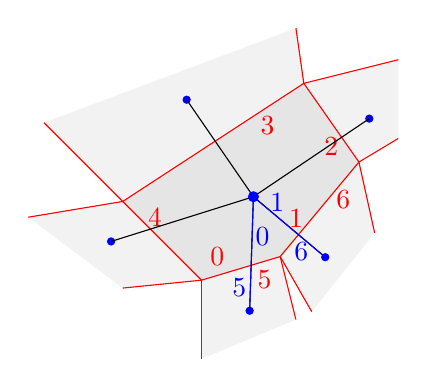
\begin{tikzpicture}
\coordinate (x0) at (0,0);
\coordinate (y0) at (-1,-.1);
\coordinate (z0) at (0,-1);

\coordinate (x1) at (1,0.3);
\coordinate (y1) at (1.2,-.5);
\coordinate (z1) at (1.4,-.4);

\coordinate (x2) at (2,1.5);
\coordinate (y2) at (2.2, 0.6);
\coordinate (z2) at (2.5, 1.8);

\coordinate (x3) at (1.3,2.5);
\coordinate (y3) at (2.5,2.8);
\coordinate (z3) at (1.2,3.2);

\coordinate (x4) at (-1,1);
\coordinate (y4) at (-2,2);
\coordinate (z4) at (-2.2,0.8);

\coordinate (p) at (barycentric cs:x0=1,x1=1,x2=1,x3=1,x4=1);
\coordinate (p01) at (barycentric cs:p=0.5,z0=1,y1=1);
\coordinate (p02) at (barycentric cs:p=0.5,z1=1,y2=1);
\coordinate (p03) at (barycentric cs:p=0.5,z2=1,y3=1);
\coordinate (p04) at (barycentric cs:p=0.5,z3=1,y4=1);
\coordinate (p05) at (barycentric cs:p=0.5,z4=1,y0=1);

\fill[gray!10] (x0) -- (x1) -- (y1) -- (z0);
\fill[gray!10] (x1) -- (x2) -- (y2) -- (z1);
\fill[gray!10] (x2) -- (x3) -- (y3) -- (z2);
\fill[gray!10] (x3) -- (x4) -- (y4) -- (z3);
\fill[gray!10] (x4) -- (x0) -- (y0) -- (z4);



\filldraw[red,fill=gray!20] (x0)
  -- node[pos=0.2,above] {0}
     node[pos=0.8,below] {5} (x1)
  -- node[pos=0.2,above] {1}
     node[pos=0.8,below] {6} (x2)
  -- node[pos=0.2,left] {2} (x3)
  -- node[pos=0.2,below] {3} (x4)
  -- node[pos=0.2,right] {4} (x0)
  -- cycle;


\foreach \ii in {0,1,...,4}
{
\draw[red] (x\ii) -- (z\ii);
\draw[red] (x\ii) -- (y\ii);
}
\foreach \ii in {1,2,...,5}
{
\fill[blue] (p0\ii) circle (1.5pt);
\draw (p) -- (p0\ii);
}

\fill[blue] (p) circle (2pt);
\draw[blue] (p)
  -- node[pos=0.35, right=-2.3] {0}
     node[pos=0.8, left=-2] {5} (p01);

\draw[blue] (p)
  -- node[pos=0.1, right] {1}
     node[pos=0.9, left] {6} (p02);
\end{tikzpicture}\end{document}
